\documentclass{report}
\usepackage{ugentstyle}

\newcommand{\answer}[1]{
		\subsubsection*{Antwoord}
			#1
}


\begin{document}
	\maketitle{Compilers - Voorbeeldexamen}
	\tableofcontents
	\chapter{Vragen}
	\newpage
\section{Grammatica - I}
	Gegeven de taal $L = \{a^mb^nc^p\}$ met $m > p$.
	\begin{enumerate}
		\item Kan een reguliere expressie gevormd worden die de woorden uit deze taal herkent? Waarom wel/niet?
		\item Maak een niet-ambigue grammatica voor taal L.
		\item Kan de taal uitgebreidt worden met de woorden waarvoor geldt $m < p$ en $m \neq p$? Geef de aangepaste grammatica.
	\end{enumerate} 

	\answer{
		\begin{enumerate}
			\item xd

		\end{enumerate}
	}


\newpage
\section{Grammatica - II}
Gegeven de grammatica:
\begin{align*}
	X & \rightarrow YaYb|ZbZa \\
	Y & \rightarrow \epsilon \\
	Z & \rightarrow \epsilon
\end{align*}
\begin{enumerate}
	\item Zoek de FIRST, FOLLOW en nullable verzamelingen.
	\item Creëer een LL(1) parser.
	\item Bepaal de toestanden van een LR(0) parser en hun overgangen en de LR(0) parsetabel.
	\item Welke van deze 2 parsers is niet ambigu? Waarom? 
\end{enumerate}

\answer{
	\begin{enumerate}
		\item 
		De productieregel $X \rightarrow YaYb|ZbZa$ is equivalent met twee productieregels $X \rightarrow YaYb$ en $X \rightarrow ZbZa$. 
		
		\begin{align*}
			1.\qquad X & \rightarrow YaYb\\
			2.\qquad X & \rightarrow ZaZb\\
			3.\qquad Y & \rightarrow  \\
			4.\qquad Z & \rightarrow 
		\end{align*}

		\begin{table}[ht]
			\centering
			\begin{tabular}{l | l | l | l }
				\hline
					& 	nullable & first & follow \\
					\hline
					X & nee & \{a, $\epsilon$\}, & / \\
					Y & ja & \{$\epsilon$\} & \{a, b\}\\ 
					Z & ja & \{$\epsilon$\} & \{a, b\}\\ 
			\end{tabular}
		\end{table}

		\item De LL(1) parsetabel:

	
		\begin{table}[ht]
			\centering
			\begin{tabular}{l | l | l}
				  & a                                          	& b \\
				  \hline
				X & $X \rightarrow YaYb$, $X \rightarrow ZaZb$ 	& \\
				Y & $Y \rightarrow \epsilon$ 					& $Y \rightarrow  \epsilon$  \\
				Z & $Z \rightarrow \epsilon$ 					& $Z \rightarrow  \epsilon$
			\end{tabular}
		\end{table}

		\item De LR(0) toestandentabel en LR(0) parsetabel:
		\begin{figure}[ht]
			\centering
			\begin{tikzpicture}[state/.style={rectangle, draw, inner sep = 2mm}]
			\node (1) [state] {
				$\begin{aligned}
					X &\rightarrow .YaYb  \\
					X &\rightarrow .ZaZb  \\
					Y &\rightarrow . \\
					Z &\rightarrow .
				\end{aligned}$};
				
			\node (2) [state, below = 1cm of 1] {$X \rightarrow Y.aYb$};
			\node (3) [state, right = 1cm of 2] {$X \rightarrow Z.aZb$};

			\node (4) [state, below = 1cm of 2] {
				$\begin{aligned}
				X &\rightarrow Ya.Yb  \\
				Y &\rightarrow . \\
			\end{aligned}$
			};
			\node (5) [state, below = 1cm of 3] {
				$\begin{aligned}
					X &\rightarrow Za.Zb  \\
					Z &\rightarrow . \\
				\end{aligned}$
				};

			\node (6) [state, below = 1cm of 4] {$X \rightarrow YaY.b$};
			\node (7) [state, below = 1cm of 5] {$X \rightarrow ZaZ.b$};

			\node (8) [state, below = 1cm of 6] {$X \rightarrow YaYb.$};
			\node (9) [state, below = 1cm of 7] {$X \rightarrow ZaZb.$};
			
			
			\draw [->] (1) -- node[xshift=0.25cm] {Y} (2);
			\draw [->] (1) -- node[xshift=0.25cm] {Z} (3);

			\draw [->] (2) -- node[xshift=0.25cm] {a} (4);
			\draw [->] (3) -- node[xshift=0.25cm] {a} (5);

			\draw [->] (4) -- node[xshift=0.25cm] {Y} (6);
			\draw [->] (5) -- node[xshift=0.25cm] {Z} (7);

			\draw [->] (6) -- node[xshift=0.25cm] {b} (8);
			\draw [->] (7) -- node[xshift=0.25cm] {b} (9);

			
			\node (label1) [anchor=north east, inner sep = 1pt] at (1.north east) {\textbf{1.}};
			\node (label2) [anchor=north east, inner sep = 1pt] at (2.north east) {\textbf{2.}};
			\node (label3) [anchor=north east, inner sep = 1pt] at (3.north east) {\textbf{3.}};
			\node (label4) [anchor=north east, inner sep = 1pt] at (4.north east) {\textbf{4.}};
			\node (label5) [anchor=north east, inner sep = 1pt] at (5.north east) {\textbf{5.}};
			\node (label6) [anchor=north east, inner sep = 1pt] at (6.north east) {\textbf{6}};
			\node (label7) [anchor=north east, inner sep = 1pt] at (7.north east) {\textbf{7.}};
			\node (label8) [anchor=north east, inner sep = 1pt] at (8.north east) {\textbf{8.}};
			\node (label9) [anchor=north east, inner sep = 1pt] at (9.north east) {\textbf{9.}};

			\end{tikzpicture}
		\end{figure}

		\begin{table}
			\centering
			\begin{tabular}{| l | l | l | l | l | l |}
				\hline
					& a & b & \$ & Y & Z \\
					\hline
				1   &   &   &    & g2&g3 \\
				2   & s4  &   &    & & \\
				3   & s5  &   &    & & \\
				4   &   &   &    & g6& \\
				5   &   &   &    & & g7\\
				6   &   & s8  &    & & \\
				7   &   & s9  &    & & \\
				8   & r1  & r1  & r1   & & \\
				9   & r2  & r2  &  r2  & & \\
				\hline
			\end{tabular}
		\end{table}

		\item De LR(0) parser is niet ambigue aangezien er geen shift-reduce conflicten aanwezig zijn. De LL(0) parser is wel ambigue omdat er meerdere productieregels kunnen toegepast worden bij het "verwerken" van de lege string.
	\end{enumerate}
}


\newpage
\section{Deterministische Eindige Automaten}
	Herschrijf de volgende deterministische eindige automaat als een reguliere expressie.
	\begin{figure}[ht]
		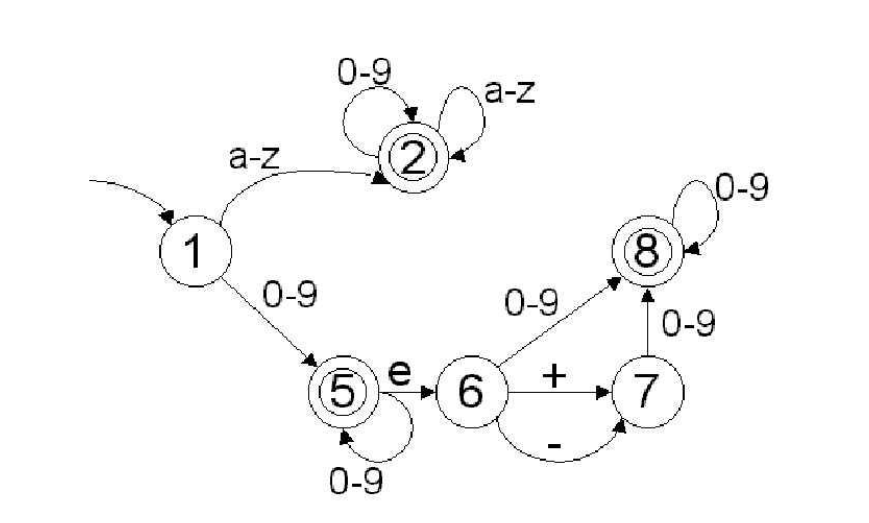
\includegraphics[width=\textwidth]{dfa_to_re}
	\end{figure}
	$$\texttt{[a-z][0-9a-z]*|[0-9]+(e[0-9|+|-][0-9]*)+}$$
	\newpage
\section{Compilerfasen - I}
	Gegeven de opeenvolgende fasen van een compiler, geef aan de programmavoorstellingen, grafen of datastructuren die aan het \textit{eind} van elke fase geproduceerd worden. Geef uw antwoord in de vorm: a-7, b-3, ...
	\begin{table}[ht]
		\begin{tabular}{l l}
			\hline
			Compilerfase & Programmavoorstelling \\
			\hline 
			(a) scanning (lexicale analyse) & 1.  intermediaire boomtaal \\
			(b) parsing  (syntactische analyse) & 2.  control flow graaf (CFG) \\
			(c) type checking (semantische analyse) & 3.  frame layout, activation records \\
			(d) vertaling (translate) & 4.  symbooltabellen \\
			(e) canonicalisering & 5.  interferentiegraaf \\
			(f) instructieselectie & 6.  gekleurde interference graph \\
			(g) controlestroom analyse & 7.  tokens \\
			(h) dataflow analyse (liveness) & 8.  assembler code \\
			(i) register allocatie & 9.  assembler instructies \\
			(j) code emission & 10.  abstracte syntax tree (AST)
		\end{tabular}
	\end{table}

	\answer{a-7, b-10, c-4, d-3, e-1, f-9, g-2, h-5, i-6, j-8}

	\newpage
	\section{Lexicale analyse}
	\label{sec:lexicale_analyse}
	
	Volgende nondeterministische eindige automaat herkent geldige tokens \texttt{(aa)+} en \texttt{(aaa)+}. 
	\begin{figure}[ht]
		\centering
		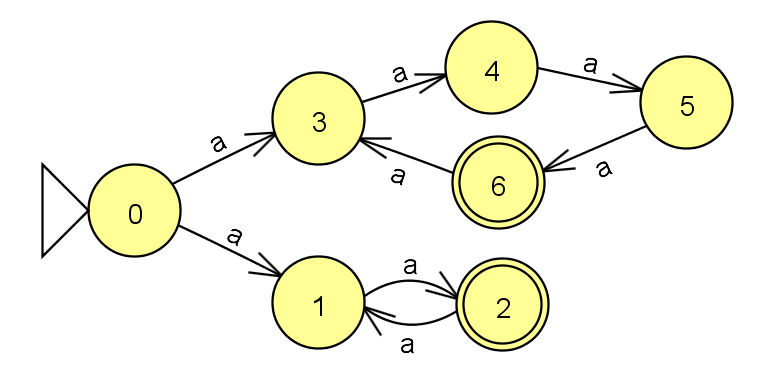
\includegraphics[width=\textwidth]{vr2_niet_deterministische_automaat}
	\end{figure}
	\begin{enumerate}
		\item Beschrijf de manier om in het algemeen verschillende NFA's samen te voegen tot 1 DFA. Bespreek daarbij de definitie van \textit{sluiting}, \textit{DFAedge} en het \textit{algoritme} dat de NFA-toestanden samenvoegt tot toestanden in een DFA.
		\item Pas dit toe op dit voorbeeld: de herkenning van twee- en drievouden van \texttt{a} en teken de bekomen DFA.
		\item Zijn er in de gevonden DFA nog equivalente toestanden die men kan vereenvoudigen?
	\end{enumerate}

	\answer{
	\begin{enumerate}
		\item Een deterministische eindige automaat (DFA) is een eindige automaat waarbij elke transitie uniek is. Het algoritme om een NFA om te vormen naar een DFA maakt enerzijds gebruik van sluitingen. De sluiting $T$ van een verzameling van toestanden $S$, of \texttt{closure(S)}, bevat alle toestanden die kunnen bereikt worden voor de lege transitie $\epsilon$ voor elke staat in $S$. Dit kan wiskundig gedefinieerd worden als:
		$$T = S \cup \bigg(\bigcup_{s \in T} edge(s, \epsilon) \bigg)$$
		waarbij \texttt{edge(s, c)} de staten geeft die vanuit $s$ via symbool $c$ kan bereikt worden.
		
		Anderzijds maakt het algoritme ook gebruik van de functie \texttt{DFAedge(d, c)}, die de staten teruggeeft die vanuit $d$ kunnen bereikt worden bij symbool $c$.
		
		\todo{verder uitleggen}
		
		\item De automaat is enkel in staat om enkelvoudige $a$ symbolen te verwerken en aangezien er geen lege strings zijn, draagt de \texttt{closure(S)} functie hier niets bij. De eerste verwerking zorgt ervoor dat staten 1 en 3 bereikt worden. Vanuit 1 kan er naar 2 gegaan worden en vanuit 3 kan er naar 4 gegaan worden. In dit geval moet dit herhaald worden tot dat er een combinatie van staten gevonden is die al eerder gecombineerd zijn. Dit is het geval als uiteindelijk de staten 6 en 2 bereikt worden. Vanuit 6 kan naar 3 gegaan worden en vanuit 2 kan naar 1 gegaan worden. Die combinatie bestaat al, en da DFA is voltooid.
			
		\begin{figure}[ht]
			\centering
			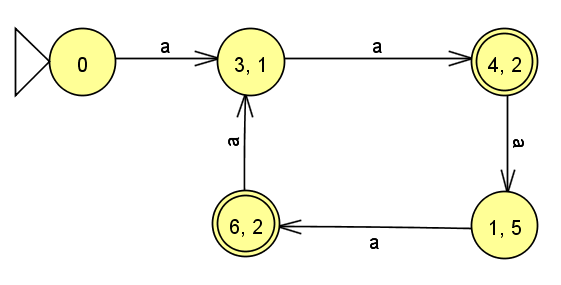
\includegraphics[width=\textwidth]{vr2_deterministische_automaat}
		\end{figure}
	
		\item Het algoritme garandeerd niet dat de opgeleverde DFA optimaal is, maar er kunnen nadien wel nog optimalisaties doorgevoerd worden. Staten die equivalent zijn kunnen samengenomen worden. Een staat $s_1$ is equivalent met staat $s_2$ als ze beiden finaal of niet finaal zijn voor dezelfde symbolen en als voor elk symbool $c$, trans[$s_1, c$] = trans[$s_1, c$]. In dit geval is dit waar voor staat $\{3, 1\}$ met $\{1, 5\}$ en voor staat $\{4, 2\}$ met $\{6, 2\}$. Deze kunnen gecombineerd worden.
		
		\begin{figure}[ht]
			\centering
			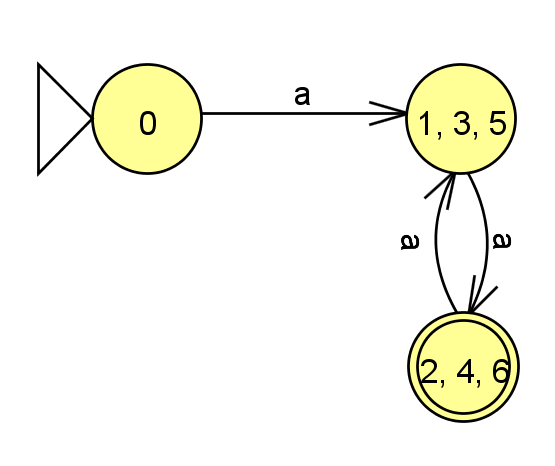
\includegraphics[width=\textwidth]{vr2_deterministische_automaat_minified}
		\end{figure}
		
		
	\end{enumerate}	
}

	\newpage
	\section{Compilerfasen - II}
	
	De volgende figuur toont de intermediaire voorstellingen die gebruikt worden als interface tussen de verschillende fasen van een compiler. Vul de nummers in van de corresponderende fasen in een compiler.
	\begin{figure}[ht]
		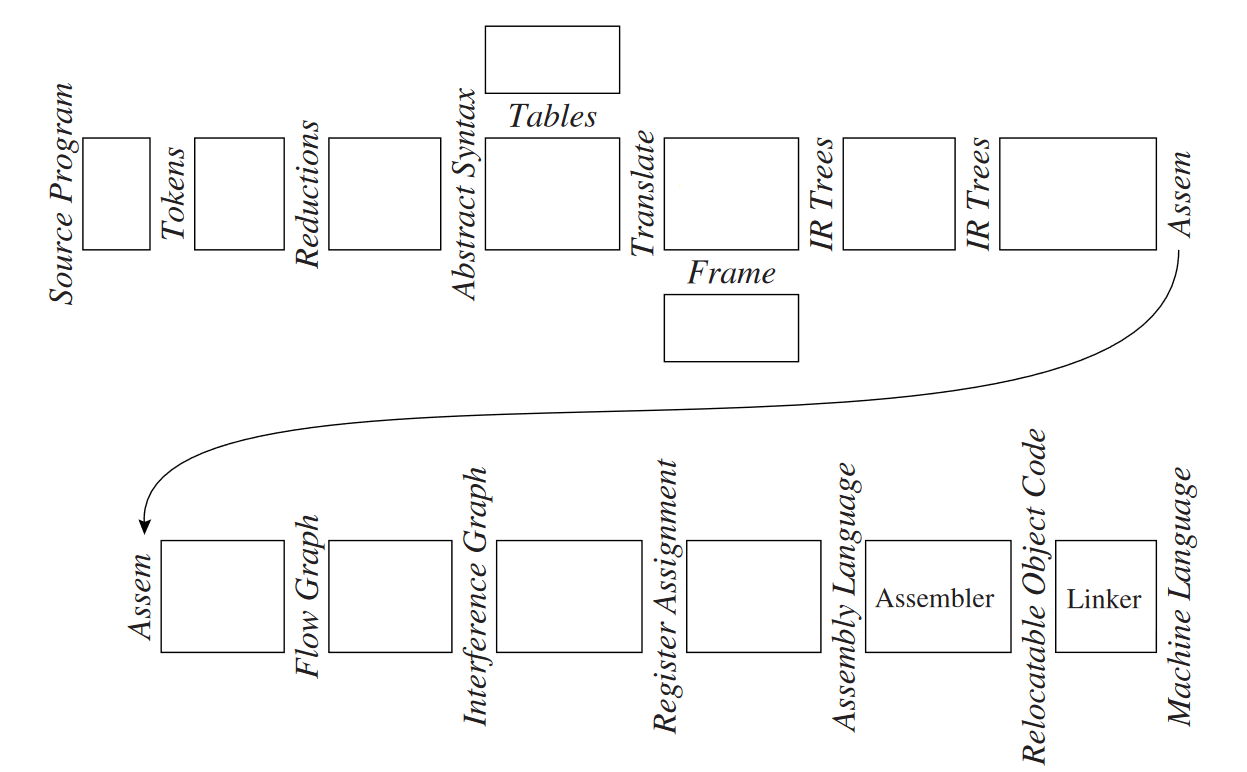
\includegraphics[width=\textwidth]{compiler_fasen}
	\end{figure}
	\begin{enumerate}
		\item Canonicalize
		\item Code Emission
		\item Control Flow Analysis
		\item Data Flow Analysis
		\item Environments
		\item Frame Layout
		\item Instruction Selection
		\item Lex
		\item Parse
		\item Parsing Actions
		\item Register Allocation
		\item Semantic Analysis
		\item Translate
	\end{enumerate}
	\answer{
		\begin{figure}[ht]
			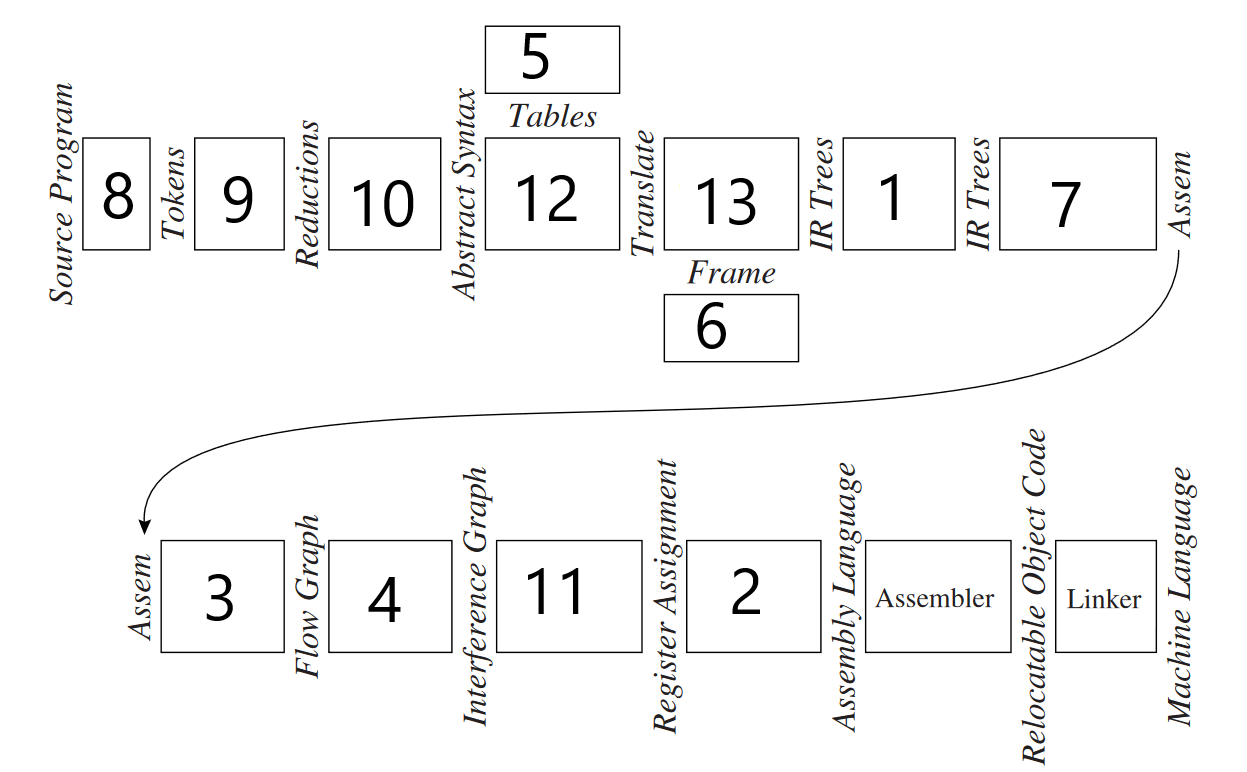
\includegraphics[width=\textwidth]{compiler_fasen_solved}
		\end{figure}
	}

	\newpage
	\section{Compilerfasen - III}
	\begin{enumerate}
		\item Onderlijn de zo goed als verplichte analyse- en transformatiestappen in een complete compiler in de onderstaande figuur. Onderlijn dus niet de optionele optimalisaties en enkel daarvoor benodigde analyses.
		\item Geef met pijlen met volle lijnen de volgorde aan waarin die verplichte stappen normaal uitgevoerd worden.
		\item Geef met pijlen met stippelijnen aan in welke volgorde en waar tussen de verplichte stappen de optionele analyses en transformaties normaal uitgevoerd worden.
	\end{enumerate}

	\newpage
	\section{Vergelijkingen}
	Bij elke set vergelijkingen passen één of meerdere termen uit onderstaand lijstje. Welke?
	\begin{enumerate}
		\item voorwaarts
		\item achterwaarts
		\item cascading analysis
		\item liveness analysis
		\item available expression analysis
		\item generational collection
		\item worklist
		\item reaching definition analysis
		\item dominator analysis
		\item initialisatie normaal gezien met lege sets
		\item initialisatie normaal gezien met volle sets
	\end{enumerate}
	\begin{table}[ht]
		\centering
		\begin{tabular}{| l | l |}
			\hline
			vergelijkingen & bijpassende termen \\
			\hline
			$in[n] = \bigcup_{p \in pred[n]} out[p]$ & 1,8,10 \\
			$out[n] = gen[n] \cup (in[n] - kill[n])$ & \\
			\hline
			$in[n] = \bigcap_{p \in pred[n]} out[p]$ & 1, 5, 11\\
			$out[n] = gen[n] \cup (in[n] - kill[n])$ & \\
			\hline
			$in[n] = use[n] \cup (out[n] - def[n])$ & 2, 4, 10\\
			$out[n] = \bigcup_{s \in succ[n]} in[s]$ & \\
			\hline
			$D[n] = \{n\} \cup \bigg(\bigcap_{p \in pred[n]} D[p]\bigg)$ & 1, 9, 11\\
			\hline
			$in[n] = gen[n] \cup (out[n] - kill[n])$ & \\
			$out[n] = \bigcup_{s \in succ[n]} in[s]$ & \\
			\hline
		\end{tabular}
	\end{table}

	\newpage
	\section{NFA}
	\begin{figure}[ht]
		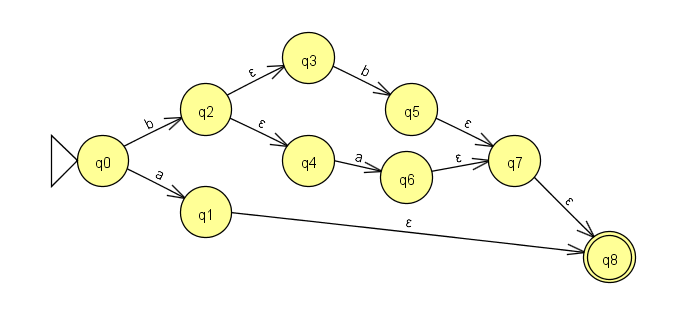
\includegraphics[width=\textwidth]{vr4_niet_deterministische_automaat}
	\end{figure}
	\begin{enumerate}
		\item Converteer deze NFA naar een DFA.
		\item Welke reguliere expressie wordt hiermee voorgesteld?
	\end{enumerate}
	\answer{
		\begin{enumerate}
			\item Gebruik dezelfde methodologie als in vraag \ref{sec:lexicale_analyse}.	\begin{figure}[ht]
				\centering
				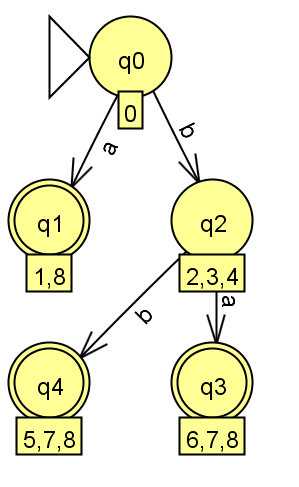
\includegraphics[width=0.5\textwidth]{vr4_deterministische_automaat}
			\end{figure}
		\item De reguliere expressie die voorgesteld wordt is $$\texttt{a+ba+bb}$$
		\todo{hoe bekomen}
		\end{enumerate}
	}

	\newpage
	\section{Parsing - I}
	Gegeven de grammatica
	\begin{align*}
	S & \mapsto E \\
	E & \mapsto E + T \\
	E & \mapsto T \\
	T & \mapsto F \\
	F & \mapsto a \\
	F & \mapsto b
	\end{align*}

	\begin{enumerate}
		\item Welke zijn de items in de initiële toestand (1) van de LR(0) parser generator?
		\item Teken de toestanden die bereikt worden na één shift of reduce actie van de LR(0) parser generator vanuit toestand 1. Teken ook de items in elke toestand.
	\end{enumerate}
	\answer{
		\begin{enumerate}
			\item 	Elke productieregel wordt een item in deze initiële toestand voor deze grammaatica.
			\begin{figure}[ht]
				\centering
				\begin{tikzpicture}[state/.style={rectangle, draw, inner sep = 2mm}]
				\node (1) [state] {
					$\begin{aligned}
					S & \mapsto .E \\
					E & \mapsto .E + T \\
					E & \mapsto .T \\
					T & \mapsto .F \\
					F & \mapsto .a \\
					F & \mapsto .b
					\end{aligned}$};
				\node (label1) [anchor=north east, inner sep = 1pt] at (1.north east) {\textbf{1.}};
				\end{tikzpicture}
			\end{figure}
			\item Vanuit de eerste toestand zijn er enkel shift acties mogelijk. 
			\begin{figure}[ht]
				\centering
				\begin{tikzpicture}[state/.style={rectangle, draw, inner sep = 2mm}]
				\node (1) [state] {
					$\begin{aligned}
					S & \mapsto .E \\
					E & \mapsto .E + T \\
					E & \mapsto .T \\
					T & \mapsto .F \\
					F & \mapsto .a \\
					F & \mapsto .b
					\end{aligned}$};
				
			\node (2) [state, above = 1.5cm of 1] {$
				\begin{aligned}
					S & \mapsto E. \\
					E & \mapsto E. + T \\
				\end{aligned}
				$};
			\node (3) [state, right = 1.5cm of 1] {$
				\begin{aligned}
				E & \mapsto T. \\
				\end{aligned}
				$};
			\node (4) [state, below = 1.5cm of 3] {$
				\begin{aligned}
				T & \mapsto F. \\
				\end{aligned}
				$};
			
			\node (5) [state, left = 1.5cm of 1] {$
				\begin{aligned}
				F & \mapsto a. \\
				\end{aligned}
				$};
			\node (6) [state, below = 1.5cm of 5] {$
				\begin{aligned}
				F & \mapsto b. \\
				\end{aligned}
				$};
			
			
			
			
			\draw [->] (1) -- node[xshift=0.25cm] {E} (2);
			\draw [->] (1) -- node[yshift=0.25cm] {T} (3);
			\draw [->] (1) -- node[yshift=0.25cm] {F} (4);
			\draw [->] (1) -- node[yshift=0.25cm] {a} (5);
			\draw [->] (1) -- node[yshift=0.25cm] {b} (6);
			
			\node (label1) [anchor=north east, inner sep = 1pt] at (1.north east) {\textbf{1.}};
			\node (label2) [anchor=north east, inner sep = 1pt] at (2.north east) {\textbf{2.}};
			
			\node (label3) [anchor=north east, inner sep = 1pt] at (3.north east) {\textbf{3.}};
			\node (label4) [anchor=north east, inner sep = 1pt] at (4.north east) {\textbf{4.}};
						
			\node (label5) [anchor=north east, inner sep = 1pt] at (5.north east) {\textbf{5.}};
			\node (label6) [anchor=north east, inner sep = 1pt] at (6.north east) {\textbf{6.}};

			\end{tikzpicture}
		\end{figure}
	\end{enumerate}}
	
	\newpage
	\section{Parsing - II}
	Gegeven de volgende context-vrije grammatica:

	
		\begin{enumerate}
			\item[0.] $S  \mapsto E\$$
			\item[1.] $E  \mapsto id$
			\item[2.] $E  \mapsto id(E)$
			\item[3.] $E  \mapsto E + id$
		\end{enumerate}

	\begin{enumerate}
		\item Bouw een LR(0) DFA voor deze grammatica.
		\item Is dit een LR(0) grammatica? Toon aan Waarom.
		\item Is dit een SLR grammatica? Toon aan Waarom.
		\item Is dit een LR(1) grammatica? Toon aan Waarom.
	\end{enumerate}
	\answer{
		\begin{enumerate}
			\item De LR(0) toestandenautomaat:
			
				\begin{figure}[ht]
				\centering
				\begin{tikzpicture}[state/.style={rectangle, draw, inner sep = 2mm}]
				\node (1) [state] {
					$\begin{aligned}
						S & \mapsto .E\$ \\
						E & \mapsto .id\\
						E & \mapsto .id(E) \\
						E & \mapsto .E + id
					\end{aligned}$};
				
				\node (2) [state, right = 1.5cm of 1] {$
					\begin{aligned}
					S & \mapsto E.\$ \\
					E & \mapsto E. + id\\
					\end{aligned}
					$};
				
				\node (3) [state, below = 1.5cm of 2] {$
					\begin{aligned}
					E & \mapsto E+.id \\
					\end{aligned}
					$};
				\node (4) [state, right = 1.5cm of 3] {$
					\begin{aligned}
					E & \mapsto E+id. \\
					\end{aligned}
					$};
				
				\node (5) [state, below = 1.5cm of 1] {$
					\begin{aligned}
					E & \mapsto id. \\
					E & \mapsto id.(E) \\
					\end{aligned}
					$};
				
				\node (6) [state, below = 1.5cm of 5] {$
					\begin{aligned}
					E & \mapsto id(.E) \\
					E & \mapsto .id \\
					E & \mapsto .id(E) \\
					E & \mapsto .E + id
					\end{aligned}
					$};
			   \node (7) [state, right = 1.5cm of 6] {$
					\begin{aligned}
					E & \mapsto id(E.) \\
					E & \mapsto E. + id
					\end{aligned}
					$};
				
				\node (8) [state, right = 1.5cm of 7] {$
					\begin{aligned}
					E & \mapsto id(E). \\
					\end{aligned}
					$};
				
				\draw [->] (1) -- node[yshift=0.25cm] {E} (2);
				\draw [->] (2) -- node[xshift=0.25cm] {+} (3);
				\draw [->] (3) -- node[yshift=0.25cm] {id} (4);
				\draw [->] (1) -- node[xshift=0.25cm] {id} (5);
				\draw [->] ([xshift=-20pt] 5.south) -- node[xshift=-0.5cm] {(} ([xshift=-20pt] 6.north);
				\draw [->] ([xshift=20pt] 6.north) -- node[xshift=0.5cm] {id} ([xshift=20pt] 5.south);
				\draw [->] (6) -- node[yshift=0.25cm] {E} (7);
				
				\draw [->] (7) -- node[xshift=0.25cm] {+} (3);
				\draw [->] (7) -- node[yshift=0.25cm] {)} (8);
				
				\node (label1) [anchor=north east, inner sep = 1pt] at (1.north east) {\textbf{1.}};
				\node (label2) [anchor=north east, inner sep = 1pt] at (2.north east) {\textbf{2.}};
				
				\node (label3) [anchor=north east, inner sep = 1pt] at (3.north east) {\textbf{3.}};
				\node (label4) [anchor=north east, inner sep = 1pt] at (4.north east) {\textbf{4.}};
				
				\node (label5) [anchor=north east, inner sep = 1pt] at (5.north east) {\textbf{5.}};
				\node (label6) [anchor=north east, inner sep = 1pt] at (6.north east) {\textbf{6.}};
				
				\node (label7) [anchor=north east, inner sep = 1pt] at (7.north east) {\textbf{7.}};
				\node (label8) [anchor=north east, inner sep = 1pt] at (8.north east) {\textbf{8.}};
				
				\end{tikzpicture}
			\end{figure}
		
			\item Dit is geen LR(0) grammatica. De LR(0) parsetabel (tabel \ref{LR0PARSETABEL})  toont aan dat er een shift-reduce conflict is in toestand 5 voor symbool (.
			\begin{table}[ht]
				\centering
				\begin{tabular}{c|ccccc|cc|}
					& id & ( & ) & + & \$ & S & E \\
					\hline 
					1 & s5 & & & & & & g2 \\
					2 & & & & s3 & a & & \\
					3 & s4 & & & & & & \\
					4 & r3 & r3 & r3 & r3 & r3 & & \\
					5 & r1 & s6, r1 & r1 & r1 & r1 & & \\
					6 & s5 & & & & & & g7 \\
					7 & & & s8 & s3 & & & \\
					8 & r2 & r2 & r2 & r2 & r2 & & \\
					\hline
				\end{tabular}
			\caption{De LR(0) parsetabel.}
			\label{LR0PARSETABEL}
			\end{table}
		
			\item Voor de SLR parsetabel moet eerst de follow set bepaald worden van elke niet-terminaal dat niet $S$ is.
			\begin{itemize}
				\item FOLLOW($E$) = + )
			\end{itemize}
			De reductie voor elke niet-terminaal moet nu enkel uitgevoerd worden voor de terminalen in de follow set. De SLR parsetabel (tabel \ref{SLRPARSETABEL}) toont aan dat er geen shift-reduce conflicten zijn. Dit is een SLR grammatica.
			\begin{table}[ht]
				\centering
				\begin{tabular}{c|ccccc|cc|}
					& id & ( & ) & + & \$ & S & E \\
					\hline 
					1 & s5 & & & & & & g2 \\
					2 & & & & s3 & a & & \\
					3 & s4 & & & & & & \\
					4 & & & r3 & r3 & & & \\
					5 & & s6 & r1 & r1 & & & \\
					6 & s5 & & & & & & g7 \\
					7 & & & s8 & s3 & & & \\
					8 & & & r2 & r2 & & & \\
					\hline
				\end{tabular}
				\caption{De SLR parsetabel.}
				\label{SLRPARSETABEL}
			\end{table}
			
			\item Als een grammatica SLR is, is het ook een LR(1) grammatica vanwege de hiërarchische ordening.  
			
		\end{enumerate}

	}
\newpage
\section{Liveness en registerallocatie}
	Gegeven volgend programma:
	\begin{lstlisting}
	1.  a = 1
	2.  b = 2
	3.  c = a + b
	4.  d = a
	5.  e = c + 2*b
	6.  f = b + e
	7.  return [d,f]
	\end{lstlisting}
	\begin{enumerate}
		\item Doe de liveness analyse.
		\item Teken de interferentiegraaf.
		\item Maak een registerallocatie via graafkleuring, met het minimum aantal registers.
	\end{enumerate}

	\answer{
		\begin{enumerate}
			\item Deel het programma op in individuele instructies en bepaal per instructie zijn succesor set, use set en def set. Pas daarna het iteratief algoritme toe om de in en out sets te berekenen.
			\begin{align*}
				in[n] & = use[n] \cup (out[n] - def[n])\\
				out[n] & = \bigcup_{s \in succ[n]} in[s]
			\end{align*}
			\begin{table}[ht]
				\centering
				\begin{tabular}{| c | c c c || l l | l l|}
					\hline
								& Succ & Use & Def & Out        	& In				\\
					\hline
					7          &  /   & d,f &  /  &            	&  d,f   			\\
					6          &  7   & b,e &  f  & d,f        	&  b,d,e		\\
					5          &  6   & b,c &  e  & b,d,e 		&  c,b,d		\\
					4          &  5   &  a  &  d  & c,b,d    	&  a,b,c			\\
					3          &  4   & a,b &  c  & a,b,c     	&  a,b		\\
					2          &  3   &  /  &  b  & a,b     	&  a    		\\
					1          &  2   &  /  &  a  & a        	&  /     		\\
					\hline
				\end{tabular}
			\end{table}
			\item De interferentiegraaf wordt bekomen door variabelen te verbinden die op hetzelfde moment live kunnen zijn (in set). De graaf is te zien op figuur \ref{fig:interferentie_graaf}
			\begin{figure}
				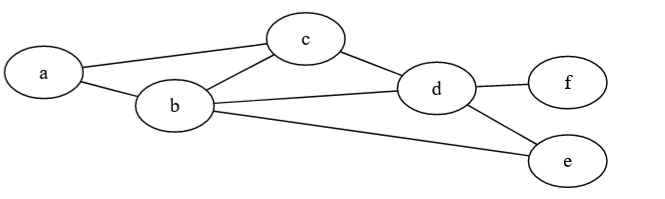
\includegraphics[width=0.5\textwidth]{interferentie_graaf}
				\caption{De interferentiegraaf.}
				\label{fig:interferentie_graaf}
			\end{figure}
			\item Er zijn minimum 3 registers nodig aangezien er zeker drie variabelen op hetzelfde moment nodig zullen zijn (afleiden uit de in set). Volgende procedure wordt uitgevoerd:
			\begin{enumerate}
				\item Simplify \textbf{f}.
				\item Simplify \textbf{e}.
				\item Simplify \textbf{d}.
				\item Simplify \textbf{c}.
				\item Simplify \textbf{b}.
				\item Simplify \textbf{a}.
				\item Select \textbf{a} - rood.
				\item Select \textbf{b} - groen.
				\item Select \textbf{c} - blauw.
				\item Select \textbf{d} - rood.
				\item Select \textbf{e} - blauw.
				\item Select \textbf{f} - groen.

			\end{enumerate}
			De resulterende graaf is te zien op figuur \ref{fig:interferentie_graaf_gekleurd}. Er kan dus afgeleidt worden dat c en d 
			\begin{figure}
				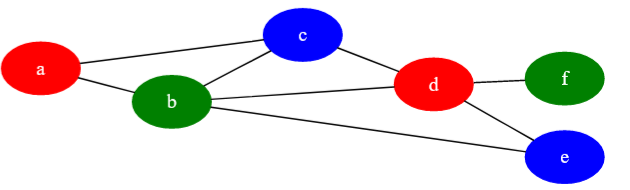
\includegraphics[width=0.5\textwidth]{interferentie_graaf_gekleurd}
				\caption{De gekleurde interferentiegraaf.}
				\label{fig:interferentie_graaf_gekleurd}
			\end{figure}
		\end{enumerate}

	}
	\newpage
\section{Registerallocatie}
	\begin{enumerate}
		\item Beschrijf kort de verschillende fasen van het registerallocatie-algoritme.
		\item Wat is de betekenis van "moves"?
		\item Hoe worden ze vermeden/weggewerkt?
		\item Geef de 2 algoritmen + tekening. 
	\end{enumerate} 
	\answer{
		\begin{enumerate}
			\item Er zijn twee varianten van het registerallocatie-algoritme. Eerst wordt het algoritme uitgelegd zonder \textit{conservative coalescing}, daarna met \textit{conservative coalescing}. Beide algoritmen hebben een restrictie op het aantal kleuren ($K$) die gebruikt mogen worden.
			\begin{enumerate}
				\item Als er geen \textit{conservative coalescing} gebruikt wordt, dan zijn er 5 fasen:
				\begin{enumerate}
					\item \textbf{Build}: deze fase stelt de interferentiegraaf op door behulp van liveness analyse.
					\item \textbf{Simplify}: Per iteratie in deze stap wordt er een knoop op een stack geplaatst en die minder dan $K$ buren heeft. Die knoop zal zeker een kleur kunnen krijgen. Deze stap wordt herhaald totdat er ofwel geen knopen meer zijn in de graaf ofwel als er geen knopen meer zijn die minder dan $K$ buren hebben.
					\item \textbf{Spill}: Als alle resterende knopen $K$ of meer buren hebben, dan wordt een willekeurige knoop gekozen om te \textit{spillen} en wordt deze ook op de stack geplaatst. Spilling zorgt ervoor dat de temporary in het geheugen bewaard zal worden in plaats van het register, dus de interferentie tussen de temporary en alle andere temporaries verdwijnt.
					\item \textbf{Select}: Vanaf dat elke knoop zich op de stack bevindt, worden ze één per één terug afgehaald en krijgen ze een kleur toegekend. Knopen die met de \textbf{simplify} opdracht op de stack geplaatst zijn kunnen zeker een kleur krijgen. Wanneer een knoop met de \textbf{spill} opdracht op de stack geplaatst wordt, is er geen garantie dat deze gekleurd kan worden. Als ze niet gekleurd kan worden praten we over een echte spill in plaats van een potentiële spill.
					\item \textbf{Start Over}: Als de \textbf{select} fase niet alle knopen heeft kunnen kleuren (door het plaatsvinden van echte spills), wordt het algoritme opnieuw uitgevoerd met een licht gewijzigd programma: de temporary die de spill veroorzaakte wordt nu in het geheugen opgeslagen na elke definitie en uit het geheugen gelezen voor elke use. Dit zorgt voor meer temporaries, maar ze hebben elk een kortere liveness range zodat ze minder interferen met andere temporaries.
				\end{enumerate}
				\item Er kan ook \textit{conservative coalescing} toegepast worden. Dit is het samenvoegen van twee move-gerelateerde knopen die het kleuren van de graaf zeker niet moeilijker zal maken. Het algoritme bevat nu twee extra stappen, alle andere stappen zijn hetzelfde als zonder \textit{conservative coalescing}:
				\begin{enumerate}
					\item \textbf{Build}
					\item \textbf{Simplify}
					\item \textbf{Coalesce:} Knopen die samen move-gerelateerd zijn kunnen samengevoegd worden. Er kunnen hier twee heuristieken gebruikt worden om knopen $a$ en $b$ samen te voegen:
					\begin{itemize}
						\item heuristiek van Briggs: als de resulterende knoop $ab$ minder dan $K$ buren heeft met $K$ of meer buren.
						\item heuristiek van George: als elke buur $t$ van $a$ ofwel een buur is van $b$ ofwel een knoop is met minder dan $K$ buren. 
					\end{itemize}
					\item \textbf{Freeze:} Wanneer zowel \textbf{simplify} als \textbf{coalesce} niet meer van toepassing zijn, kunnen de move-gerelateerde knopen bevrozen worden. Dit komt er op neer dat de move-interferentie tussen elke andere knoop die buur is verwijdert wordt, zodat de graaf vereenvoudig is.
					\item \textbf{Spill}
					\item \textbf{Select}
					\item \textbf{Start Over}
				\end{enumerate}
			\end{enumerate}
			\item Een move komt voor wanneer een temporary naar een andere temporary gekopieerd wordt: $t \leftarrow z$. 
			\item Via het registerallocatie-algoritme met \textit{conservative coalescing} kunnen zulke operaties weggewerkt worden. Inderdaad, knopen die \textit{gecoalesced} zijn krijgen hetzelfde register toegewezen. 
			\begin{align*}
				z &\leftarrow x \oplus y \\
				t &\leftarrow z 
			\end{align*}
			In dit geval zullen $z$ en $t$ hetzelfde register krijgen (bv $r3$):
			\begin{align*}
				r3 &\leftarrow x \oplus y \\
				r3 &\leftarrow r3 
			\end{align*}
			zodat de laatste toekenning geschrapt kan worden.

			\item 
			\begin{itemize}
				\item Registerallocatie zonder \textit{conservative coalescing}.
				\begin{figure}[ht]
					\centering
					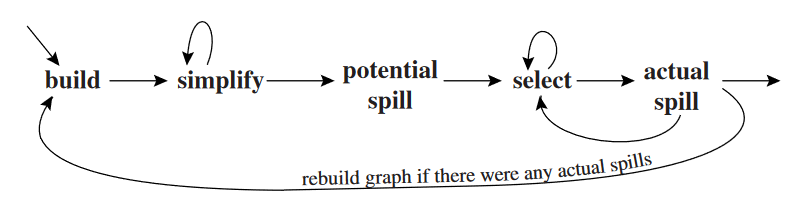
\includegraphics[width=\textwidth]{registerallocatie_nocoalescing}
				\end{figure}
				\item Registerallocatie met \textit{conservative coalescing}.
				\begin{figure}[ht]
					\centering
					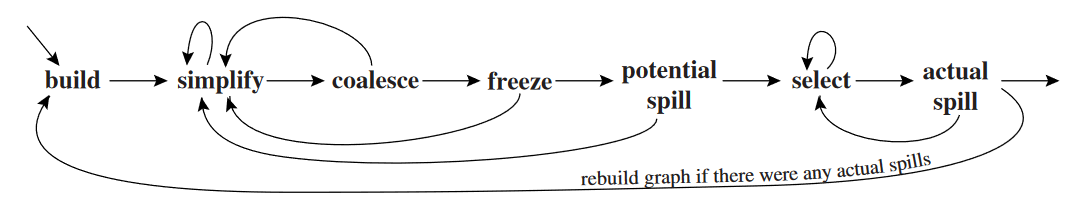
\includegraphics[width=\textwidth]{registerallocatie_coalescing}
				\end{figure}
			\end{itemize}

		\end{enumerate}
	}
	\newpage
\section{Bevriezen}
	 In welke fase van de compiler wordt de term bevriezen (freeze) gebruikt? Wanneer wordt deze techniek toegepast, en wat is het nut ervan?
	 \answer{
		Bevriezen heeft betrekking tot registerallocatie. In de interferentiegraaf kunnen move-gerelateerde verbindingen zijn. Wanneer een knoop met een move-gerelateerde verbinding bevrozen wordt, worden alle move-gerelateerde verbindingen van die knoop verwijderd. Dit heeft als gevolg dat eventueel de move operatie twee verschillende registers nodig heeft. Het wordt gebruikt om de interferentiegraaf eenvoudiger te maken.
	 }
	 \newpage
\section{Bereikende definities}
	\begin{enumerate}
		\item Wat zijn bereikende definities (reaching definitions)?
		\item Wat zijn de gen- en kill-verzamelingen voor de statements voor volgende types van statements?
		\begin{table}[ht]
			\centering
			\begin{tabular}{l l l}
				Statement $s$ & gen[s] & kill[s] \\
				\hline
				$d : t \leftarrow b \oplus c$ & & \\
				$d : t \leftarrow M[b]$  & & \\
				$M[a] \leftarrow b$  & & \\
				if $a$ relop $b$ goto $L_1$ else goto $L_2$  & & \\
				goto $L$  & & \\
				$L :$  & & \\
				$f(a_1, ... , a_n)$  & & \\
				$d : t \leftarrow f(a_1, ..., a_n)$  & & \\
			\end{tabular}
		\end{table}
		\item Worden reaching definities gebruikt bij
		\begin{enumerate}
			\item eliminatie van gemeenschappelijke subexpressies?
			\item copy propagatie?
			\item dode code eliminatie?
		\end{enumerate}
		Geef alle mogelijkheden. Verklaar uw antwoord, zo mogelijk met een voorbeeld.
		\item Geef de vergelijkingen van de in- en out-verzamelingen voor een statement $n$.
		\item Gegeven twee opeenvolgende statements $p$ en $n$ in een basisblok. Bereken de vergelijkingen van de in- en out-verzamelingen van het blok $pn$ van de tweede opeenvolgende statements.
	\end{enumerate}
	\answer{
		\begin{enumerate}
			\item Een reaching definition voor een statement $n$ zijn alle statements $s_i$ die een waarde toekennen aan een temporary, waarbij de waarde nog steeds beschikbaar is in $n$. 
			\item 		
			Stel $defs(t)$ alle statements waarin $t$ gedefinieerd wordt:
			\begin{table}[ht]
				\centering
				\begin{tabular}{l l l}
					Statement $s$ & gen[s] & kill[s] \\
					\hline
					$d : t \leftarrow b \oplus c$ & \{d\} & defs(t) - \{d\} \\
					$d : t \leftarrow M[b]$  & \{d\} & defs(t) - \{d\} \\
					$M[a] \leftarrow b$ & \{\} & \{\} \\
					if $a$ relop $b$ goto $L_1$ else goto $L_2$  & \{\} & \{\} \\
					goto $L$  & \{\} & \{\} \\
					$L :$  & \{\} & \{\} \\
					$f(a_1, ... , a_n)$  & \{\} & \{\} \\
					$d : t \leftarrow f(a_1, ..., a_n)$  & \{d\} & defs(t) - \{d\} \\
				\end{tabular}
			\end{table}
			\item 
			\begin{enumerate}
				\item Nee. 

				Een reaching definition heeft enkel betrekking tot definities van temporaries. Om gemeenschappelijke subexpressies te elimineren moeten de reaching expressions bepaald worden. Een expressie $t \leftarrow x \oplus y$ (binnen een knoop $s$) bereikt een knoop $n$ als er een pad bestaat van $s$ naar $n$ waarbij er in geen enkele knoop op dat pad een  toekenning is aan $x$ of $y$.

				\item Ja.

				Een definitie $n : t \leftarrow t \oplus x$ en $d : t \leftarrow z$  kan vervangen worden door $n : t \leftarrow z \oplus x$ als er een pad bestaat van $d$ naar $n$ en als er geen andere definitie van $t$ statement $n$ bereikt. 
				
				\item Nee.

				Dode code elmination verwijdert statements die nergens gebruikt worden. Stel een definitie $s : a \leftarrow b$. Als $a$ niet live-out $s$ is, dan kan $s$ verwijderd worden. Dit wordt geïmplementeerd via de out-verzamelingen bij liveness analyse.
			\end{enumerate}
			\item Voor een statement $n$ zijn de vergelijkingen van de in- en out-verzamelingen
			\begin{align*}
				in[n]  &= \bigcup_{p \in pred[n]} out[p] \\
				out[n] &= gen[n] \cup (in[n] - kill[n])
			\end{align*}
			Hierbij is $pred[n]$ de verzameling statements die $n$ als directe opvolger hebben.

			\item Als $p$ de enige voorganger is van $n$, dan kan eerst de vergelijking opnieuw geschreven worden:
			\begin{align*}
				out[n] &= gen[n] \cup (in[n] - kill[n]) \\
				in[n] & = out[p] = gen[p] \cup (in[p] - kill[p])\\
				out[n] & = gen[n] \cup ((gen[p] \cup (in[p] - kill[p])) - kill[n]) \\
				out[n] & = gen[n] \cup (gen[p] - kill[n]) \cup (in[p] - (kill[p] \cup kill[n]))
			\end{align*}
			Dus de vergelijkingen worden:
			\begin{align*}
				in[pn] & = gen[p] \cup (in[p] - kill[p])\\
				out[pn] & = gen[pn] \cup (in[pn] - kill[pn])
			\end{align*}
		\end{enumerate}
	}
		\newpage
\section{Constantenpropagatie}
	Veronderstel een statement $d : t \leftarrow c$ met $c$ een constante. Een ander statement $n$ gebruikt $t$, zoals in $n : y \leftarrow t \oplus x$. Onder welke voorwaarden mag men statement $n$ herschrijven als $y \leftarrow c \oplus x$?
	\begin{enumerate}
		\item Geef de precieze voorwaarden.
		\item Definieer de gebruikte termen.
	\end{enumerate}
	\answer{
		\begin{enumerate}
			\item Statement $d$ moet in eerste geval statement $n$ bereiken. Verder mag er geen andere definitie van $t$ statement $n$ bereiken.
			\item Om te bepalen of een andere definitie van $t$ statement $n$ bereikt, worden \textit{reaching definitions} gebruikt. Dit is de verzameling van statements $s_i$, waarvan de waarde van de variabele die gedefinieerd wordt door dat statement, bereikt kan worden in $n$.  
		\end{enumerate}
	}
\end{document}
